% LTeX: language=sl-SI
\section{Uvod}
% Napišite kratek zgodovinski in matematični uvod.  Pojasnite motivacijo za problem, kje
% nastopa, kje vse je bil obravnavan. Na koncu opišite tudi organizacijo dela -- kaj je v
% katerem razdelku.
Odkar se je na svetu pojavil koncept (ročnega) podpisa, je večina primerov uporabe temeljila na
pridobivanju podpisov več deležnikov, saj je bila večina podpisanih dokumentov sporazum ali pogodba
med večimi deležniki. Odličen primer je npr.\ Deklaracija neodvisnosti Združenih držav
Amerike, vidna na sliki~\ref{fig:declaration}. 

\begin{figure}[ht]
  \centering
  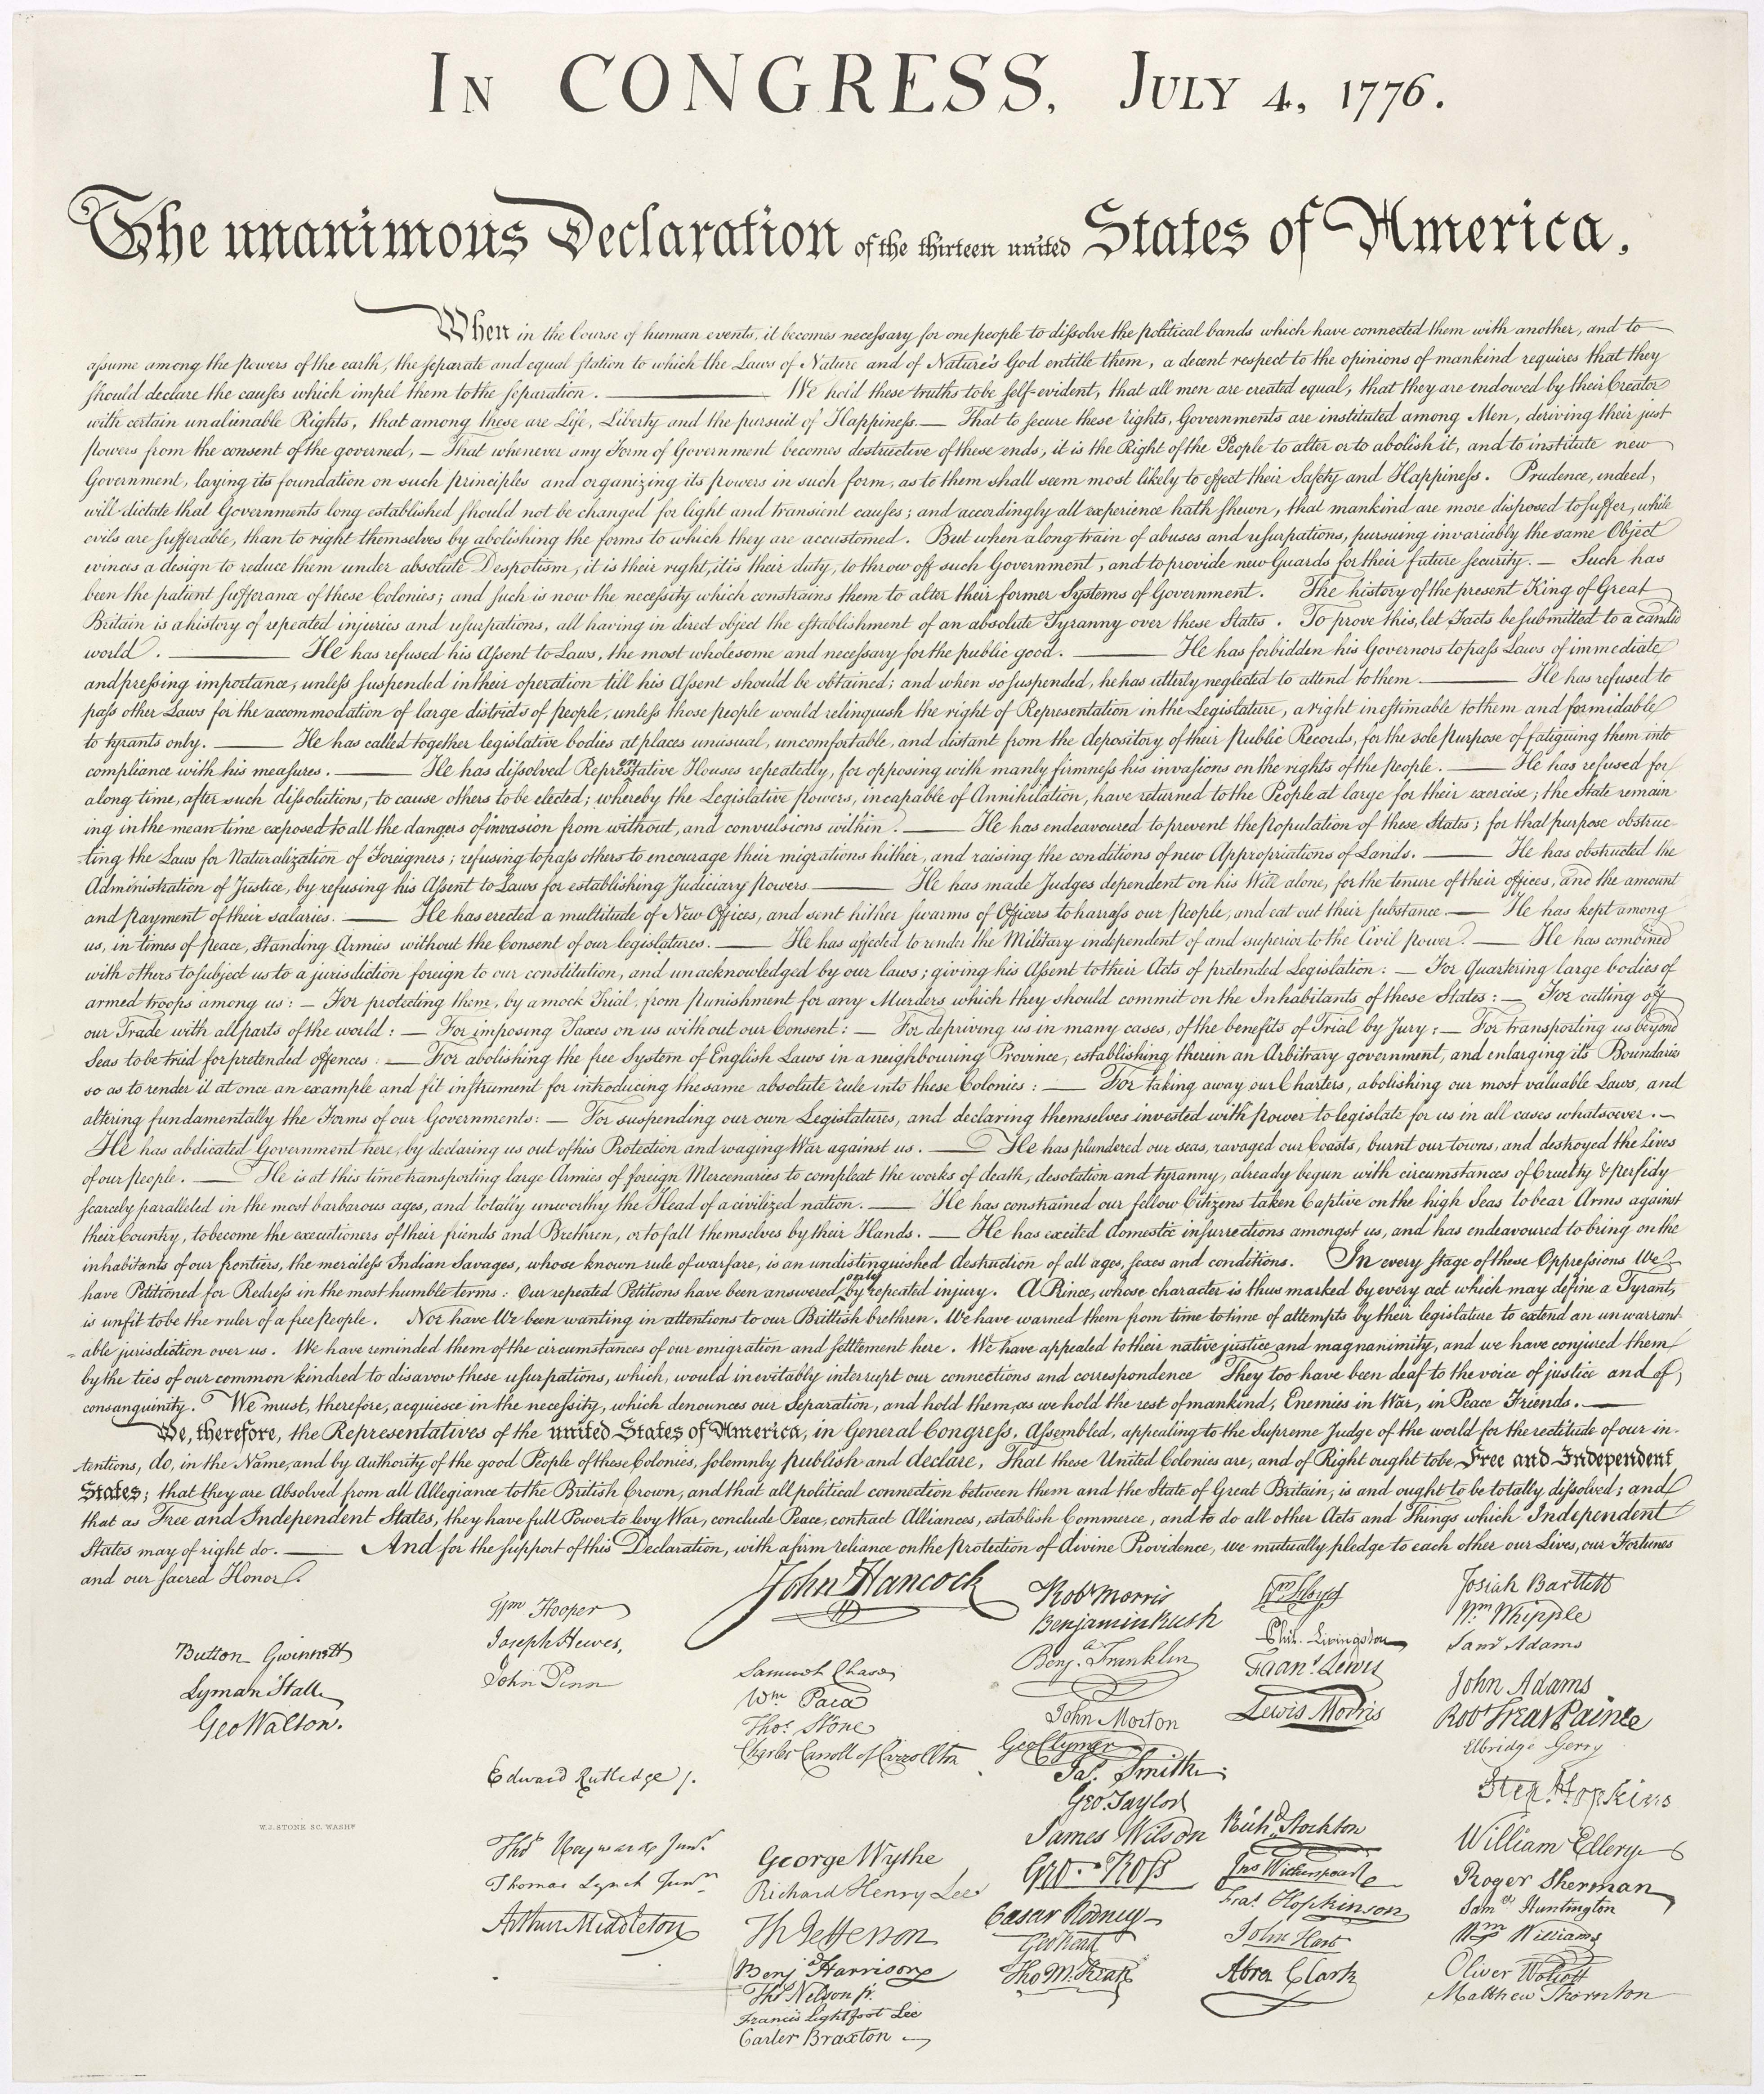
\includegraphics[width=0.5\textwidth]{images/declaration.jpg}
% \caption[caption za v kazalo]{Dolg caption pod sliko}
  \caption[Deklaracija neodvisnosti Združenih držav Amerike.]{Deklaracija neodvisnosti Združenih 
  držav Amerike s podpisi podpornikov spodaj. Vir slike Wikipedia~\cite{doi}.}
  \label{fig:declaration}
\end{figure}

S pojavom računalnika in napredkom v kriptografiji se je pojavila alternativna oblika podpisovanja.
\textit{Digitalni podpisi} so dandanes povsod. Uporabljeni so vsakič, ko dostopamo do spletnih
strani, prenašamo podatke ali pa opravljamo kakršnakoli plačila. Poleg avtomatiziranih podpisovanj,
ki se zgodijo v ozadju zgoraj omenjenih procesov, pa so digitalni podpisi na voljo tudi kot alternativa
ročnemu podpisu človeka. V praktično vseh pogledih so mnogo varnejši od tradicionalnih podpisov,
omogočajo bolj sistematično preverjanje (prek računalnikov) in so skorajda enostavnejši za uporabo
in prenašanje.

Digitalne podpise sta si prvič zamislila Diffie in Martin Hellman leta $1976$~\cite{diffie1976new},
ko sta predvidevala, da lahko take sisteme ustvarimo na podlagi enosmernih funkcij in asimetrične
kriptografije. Prvi digitalni podpis, ki je bil dejansko implementiran in široko uporabljen, pa je
bil \textit{RSA} podpis, ki so si ga leta $1977$ zamislili Ronald Rivest, Adi Shamir in Leonard
Adleman~\cite{rivest1978rsa}.

Poleg individualnih podpisov, pa lahko digitalne podpise uporabimo tudi za podpisovanje skupin, npr.\
če mora skupina deležnikov podpisati pogodbo. Najenostavneje to dosežemo tako, da vsak član pripne
svoj digitalni podpis. Če je skupina velika, če je računska moč omejena (npr.\ če želimo zmanjšati
ceno transakcij pri tehnologiji veriženja blokov), ali pa če enostavno želimo preverjevalcu podpisov
olajšati delo, lahko poskrbimo, da se skupina podpiše z enim samim, \textit{večstranskim} podpisom.
Ta podpis vseeno priča o vseh podpisnikih, njegova verifikacija oz.\ preverjanje pa zajema približno
enako dela, kot preverjanje enega samega podpisa.

Taki podpisi so samo en izmed možnih načinov, kako se skupina podpiše. Od ostalih načinov izstopajo
po tem, da omogočajo vpogled v sestavo skupine podpisnikov, kar nudi preverjevalcu več informacij
pri odločanju, če je podpis sprejemljiv, hkrati pa ohranja odgovornost individualnih članov skupine.
Pri tradicionalnih skupinskih podpisih podpis samo priča o podpisu celotne skupine, ustvari pa ga
lahko katerkoli član. Take lastnosti so v določenih primerih zelo zaželene, npr.\ pri tehnologiji
veriženja blokov je zelo pomembno, da je znano iz katerih naslovov prihajajo transakcije. To, v
kombinaciji s popularizacijo Schnorrovega podpisa, je privedlo mnogo raziskovalcev do želje po
večstranskih podpisih, ki vrnejo navadne Schnorrove podpise, in so tako enostavno zamenljivi.

Prva sta si večstranske podpise zamislila Itakura in Nakamura leta $1983$~\cite{itakura1983multi},
vendar takrat še niso videli veliko uporabe. Velik napredek je bil dosežen, ko si je Schnorr leta
$1989$ zamislil Schnorrov podpis~\cite{schnorr1989sig}, ki se je izkazal za posebno primernega za
večstranske podpise. Še vedno pa so bili takšni podpisi zanimivi bolj iz teoretičnega vidika. Leta
$2001$ se je pojavil prvi formalni model in dokaz varnosti za večstranske podpise, zahvaljujoč
Micaliju, Ohti in Reyzinu~\cite{micali2001asm}. Prvi primer široke uporabe se je pojavil z
Bitcoinom~\cite{nakamoto2009bitcoin}. Njegova popularnost je tudi popularizirala raziskovanje
večstranskih podpisov, leta $2020$ je izšel podpis MuSig2~\cite{jonas2020musig2}, ki je bil prvi
večstranski podpis, ki je bil primerno učinkovit za uporabo v Bitcoin omrežju. Široko je uporabljen
še danes.

V poglavju~\ref{sec:osnove} najprej predstavimo kriptografske osnove, ki so potrebne za razumevanje besedila.
To zajema modularno aritmetiko in grupe, zgoščevalne funkcije, kriptografijo javnega ključa, nekaj
splošnih definicij pri digitalnih podpisih in potem še nekaj besed o varnosti. V poglavju~\ref{sec:schnorr}
predstavimo Schnorrov podpis, ki je osnova za ostale sheme, ki jih obravnavamo. V 
poglavju~\ref{sec:skpine} predstavimo nekaj možnih pristopov za podpisovanje skupin. Poglavje~\ref{sec:multischnorr}
predstavi večstranski Schnorrov podpis, tam tudi dokažemo njegovo varnost v modelu slučajnega oraklja.
V poglavju~\ref{sec:primerjava} primerjamo učinkovitost navadnega in večstranskega Schnorrovega podpisa.
Na koncu pa v poglavju~\ref{sec:sodobno} omenimo še, kako se je področje razvijalo v zadnjem času.
